\documentclass[../main.tex]{subfiles}
\begin{document}\label{chap5}

Chương này thực hiện đánh giá kết quả của hai bài toán tối ưu \eqref{self} và \eqref{competitive} đã đề cập trong Chương \ref{chap4} thông qua quá trình mô phỏng với dữ liệu ngẫu nhiên. Đồng thời, hiệu năng hệ thống trong hai chiến lược này cũng được so sánh. Ngoài ra, chương này cũng đánh giá các hiệu năng của các bên trong mô hình hệ thống mở rộng, với nhiều SU cạnh tranh với nhau.

\section{Các tham số thí nghiệm}

Trong các thử nghiệm, giá trị của một số tham số sau là cố định cho tất cả các trường hợp. Mật độ phổ công suất nhiễu tại các bên nhận được cố định là $\mathcal{N}_0 = 4.0\times10^{-21}\text{ W/Hz}$, với công suất phát tối đa cho các bên $20\mathcal{N}_0 \text{ W/Hz}$. Tốc độ mã hóa tại các bên được thiết lập là $R_b^{(P)} = 1.0 \ \text{bps/Hz}$, $R_b^{(S)} = 1.0\ \text{bps/Hz}$ và tốc độ truyền tin tương ứng $R_s^{(P)} = 0.8\ \text{bps/Hz}$, $R_s^{(S)} = 0.8\ \text{bps/Hz}$.

Nhằm đánh giá ảnh hưởng của hiệu ứng suy giảm theo khoảng cách (path loss) tới các hiệu năng của hệ thống, các thử nghiệm số liệu trong đồ án này được tiến hành với giả thiết trung bình các độ lợi kênh truyền chỉ phụ thuộc vào khoảng cách giữa bên phát và bên nhận, theo công thức:
\begin{equation}\label{genomega}
    \Omega_X = \Omega_0d^{-\alpha},
\end{equation}
với $d$ là khoảng cách giữa bên phát và bên nhận (đơn vị mét, $\text{m}$), $\Omega_0$ là trung bình độ lợi kênh truyền tại khoảng cách $1\text{m}$ và $\alpha$ là hệ số suy giảm. Trong các thử nghiệm, $\alpha = 3.5$ và $\Omega_0$ được chọn để đảm bảo tỷ số tín hiệu trên nhiễu SNR (không bao gồm can nhiễu) tại khoảng cách $20 \text{m}$ là $5 \text{dB}$, khi bên phát truyền tin với công suất phát là $10\mathcal{N}_0 \text{ W/Hz}$.

Dễ thấy rằng, theo công thức \eqref{power:range}, điều kiện kênh truyền cũng ảnh hưởng đến xác suất truyền tin tối đa mà các bên có thể đạt được. Do đó, thay vì xác định giá trị tuyệt đối cho xác suất truyền tin tối thiểu $\sigma^{(P)}$ và $\sigma^{(S)}$, các bên sẽ lựa chọn hai giá trị $\rho^{(P)}$ và $\rho^{(S)}$, phản ánh tỷ lệ xác suất truyền tin cần đạt được so với xác suất truyền tin cực đại, cụ thể:
\begin{equation}
\begin{aligned}
    \sigma^{(P)} &= \rho^{(P)}\max\left\{p_{tx}^{(P)}\right\}, \\
    \sigma^{(S)} &= \rho^{(S)}\max\left\{p_{tx}^{(S)}\right\},
\end{aligned}
\end{equation}
với $\max\left\{p_{tx}^{(P)}\right\}, \max\left\{p_{tx}^{(S)}\right\}$ xác định trong \eqref{power:range}. Nếu như không đề cập cụ thể, các giá trị này mặc định là $\rho^{(P)} = 0.5$ và $\rho^{(S)} = 0.5$.

Về phương pháp giải quyết bài toán tối ưu, đồ án sử dụng giải thuật tiến hóa vi phân DE, với chiến lược DE/rand/1/bin, tức là cá thể mục tiêu được lựa chọn ngẫu nhiên (rand) với một cặp cá thể dùng làm đại lượng đột biến và chiến lược lai tạo là lai tạo đồng bộ (uniform crossover). Trong các thử nghiệm, kích thước quần thể được thiết lập là $NP=20$ với biên độ đột biến $F=0.5$ và tốc độ lai tạo $CR=0.9$. Điều kiện dừng cho thuật toán DE xác định dựa trên số lượng thế hệ tối đa, $G_{max}=50$.

\section{Phương pháp thí nghiệm}

Phương pháp thí nghiệm được sử dụng trong đồ án là Monte Carlo với $200000$ mẫu thử nghiệm. Trong các kết quả khác nhau, khi áp dụng các điều kiện lọc khác nhau, số lượng mẫu thử nghiệm có thể khác số lượng mẫu tổng cộng. Do đó, trong từng kết quả, số lượng mẫu thử nghiệm sẽ được thể hiện cụ thể theo tham số $N$.

Mỗi mẫu thử nghiệm tương ứng với một bộ các khoảng cách giữa từng cặp đối tượng thu-phát trong hệ thống. Các mẫu thử nghiệm được sinh ngẫu nhiên độc lập trong dải giá trị từ $\left[1, R_0\right]$. Giá trị $R_0$ được cố định là $30\text{m}$ trong tất cả thử nghiệm. Độ lợi kênh trung bình $\Omega_X$ tương ứng với từng khoảng cách sẽ được tính theo công thức $\eqref{genomega}$. Các kết quả thử nghiệm hầu hết đều biểu diễn theo hàm phân phối tích lũy thực nghiệm (empirical CDF), biểu diễn phân bố các giá trị dưới một ngưỡng.

\section{Điều kiện ràng buộc về xác suất truyền tin trong trường hợp hợp tác}

Trước khi trình bày chi tiết các kết quả về hai bài toán chính của đồ án, phần này đánh giá các điều kiện ràng buộc về xác suất truyền tin trong các bài toán này. Các tham số $\sigma^{(P)}$ (hay $\rho^{(P)}$) và $\sigma^{(S)}$ (hay $\rho^{(S)}$) có tác động lớn tới điều kiện khả thi của các bài toán tối ưu. Hình~\ref{fig:Feasibility:rho} thể hiện tác động của ngưỡng xác suất truyền tin yêu cầu tại SU và PU ($\rho^{(S)}$ và $\rho^{(P)}$) tới xác suất có nghiệm của bài toán tối ưu \eqref{moop}. Kết quả chỉ ra rằng, khi PU và SU càng đặt ra yêu cầu cao về xác suất truyền tin của mình thì bài toán tối ưu này càng ít cơ hội có nghiệm, tức là SU càng ít khả năng được hợp tác. Điều này hoàn toàn dễ hiểu vì xác suất truyền tin phụ thuộc vào điều kiện kênh truyền từ bên phát tới bên thu, trong đó có cả đường truyền can nhiễu. Yêu cầu ngưỡng xác suất tối thiểu quá cao đồng nghĩa loại bỏ những điều kiện kênh truyền không tốt, từ đó mà giảm cơ hội một điều kiện truyền tin bất kỳ đạt được yêu cầu đó. 

Dựa trên công thức về tốc độ lộ tin trung bình tại các bên \eqref{rlp} và \eqref{rls}, thấy rằng các giá trị này không phụ thuộc vào các kênh truyền $h_{pp}$, $h_{ps}$, $h_{sp}$ và $h_{ss}$, tức là các tham số $\rho^{(P)}$ và $\rho^{(S)}$ chỉ ảnh hưởng đến xác suất truyền tin mà không ảnh hưởng đến các hiệu năng an toàn trong các bài toán \eqref{self} và \eqref{competitive}. Do đó, trong các thử nghiệm ở phần sau, dữ liệu được sinh luôn thỏa mãn các điều kiện ràng buộc về xác suất truyền tin. Cũng theo kết quả từ Hình~\ref{fig:Feasibility:rho}, bộ tham số $\rho^{(P)} = 0.5, \rho^{(S)} = 0.5$ cho khoảng $50\%$ trường hợp dữ liệu sinh là hợp lệ.

\begin{figure}
\centering
\captionsetup{justification=centering}
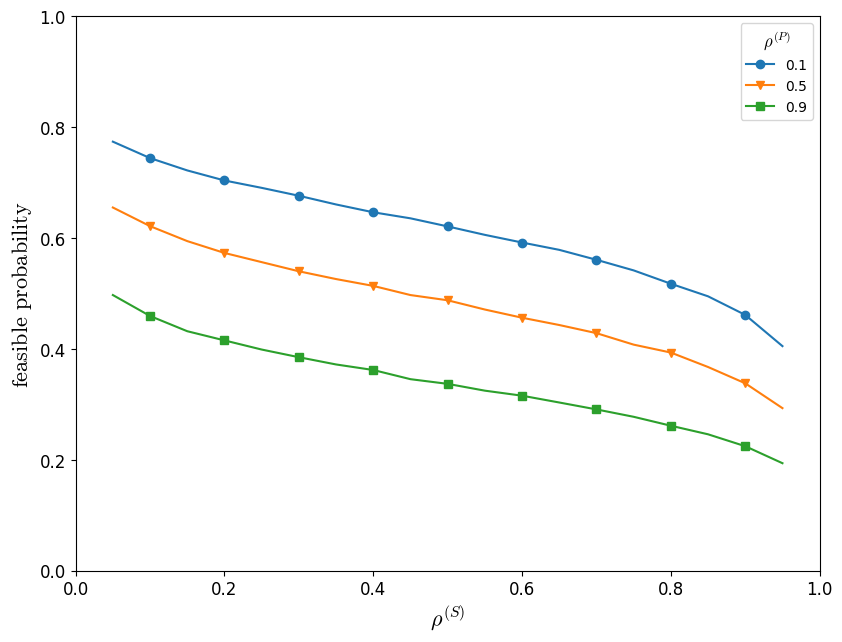
\includegraphics[width=0.8\linewidth]{sigmaS-rho-feasible.png}
\caption{Ảnh hưởng của xác suất truyền tin tối thiểu tới điều kiện khả thi của các bài toán tối ưu. $N = 50000$}
\label{fig:Feasibility:rho}
\end{figure}

\section{So sánh giữa các bài toán đề xuất}

Để so sánh hiệu năng hệ thống giữa các bài toán đề xuất, phần này tạm thời bỏ qua các điều kiện ràng buộc \eqref{self:popt}, \eqref{competitive:sopt} liên quan đến tốc độ lộ tin trung bình trong "bài toán tối ưu cá nhân" \eqref{self} và "bài toán cạnh tranh" \eqref{competitive}. Phần này thực hiện đánh giá hiệu năng tại PU trong ba trường hợp: (i) tối ưu tốc độ lộ tin trung bình $R_L^{(NC)}$ \eqref{lemmaEZ:EZNC} khi chỉ có PU truyền tin ($NC$), (ii) ưu tiên tối ưu cho SU ($SF$), là bài toán \eqref{self} không bao gồm ràng buộc \eqref{self:popt} và (iii) ưu tiên tối ưu cho PU ($CP$), là bài toán \eqref{competitive}
không bao gồm ràng buộc \eqref{competitive:sopt}. Có thể thấy rằng với ba chiến lược này, kết quả đánh giá hiệu năng an toàn của SU cũng có thể phát biểu tương tự vì tính đối xứng giữa hai chiến lược $SF$ và $CP$. Cũng chú ý rằng, điều kiện ràng buộc \eqref{self:popt} của "bài toán tối ưu cá nhân" tương ứng với việc so sánh giữa hai chiến lược $SF$ và $NC$. Như vậy, kết quả trong phần này cũng phản ánh điều kiện hợp tác giữa PU và SU.

Hình~\ref{fig:Compare:rlp} so sánh tốc độ lộ tin trung bình tại PU trong ba trường hợp, $NC$, $SF$ và $CP$, tương ứng với ba chiến lược tối ưu khác nhau. Khi so sánh giữa hai trường hợp ưu tiên tối ưu cho PU là $NC$ (không hợp tác) và $CP$ (hợp tác với SU), ta thấy rằng việc hợp tác với SU giúp PU đạt được trung bình tốc độ lộ tin nhỏ hơn nhiều so với trường hợp không hợp tác. Tuy nhiên, việc hợp tác này không đem lại hiệu quả cho PU nếu như SU chỉ tập trung tối ưu cho lợi ích của mình, tương ứng với trường hợp $SF$.

\begin{figure}
\centering
\captionsetup{justification=centering}
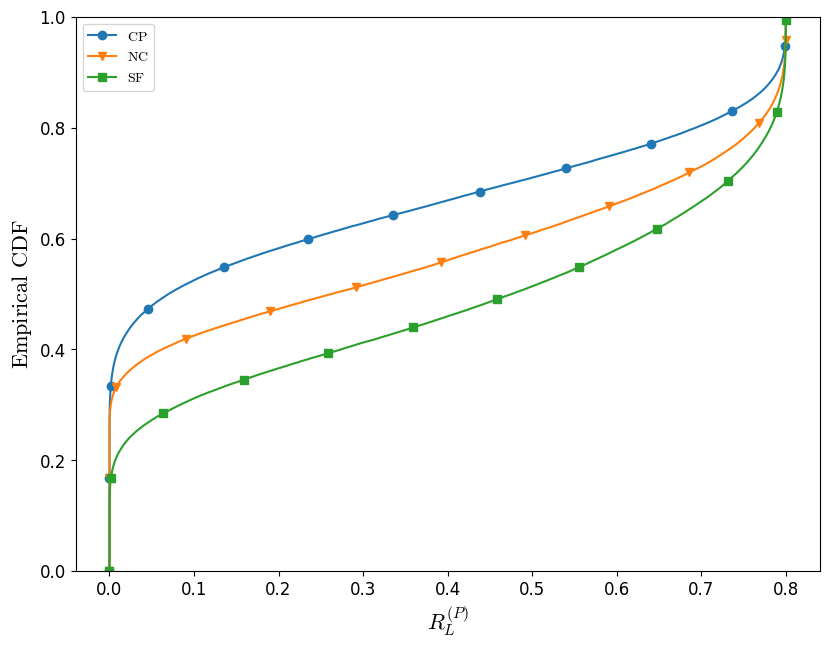
\includegraphics[width=0.8\linewidth]{compare-rlp.png}
\caption{So sánh tốc độ lộ tin trung bình tại PU giữa các chiến lược tối ưu khác nhau. $N=200000$}
\label{fig:Compare:rlp}
\end{figure}

Mặt khác, khi đánh giá hiệu năng của PU theo xác suất truyền tin $p_{tx}^{(P)}$, kết quả thu được trong Hình~\ref{fig:Compare:ptxp} cho thấy điều ngược lại. Lúc này xác suất truyền tin của PU trong chiến lược $SF$ lại cao hơn nhiều so với hai chiến lược còn lại: có đến $60\%$ các trường hợp trong $NC$ và $CP$ ở đó xác suất truyền tin dưới $50\%$, nhưng chỉ có khoảng $20\%$ trường hợp xác suất truyền tin trong $SF$ là dưới $50\%$. Do các kết quả thử nghiệm được đánh giá trên cùng tập mẫu, tức là cùng điều kiện kênh truyền, nên kết quả này phản ánh đặc điểm giá trị công suất phát tối ưu trong các trường hợp đó. Với cùng điều kiện kênh truyền và điều kiện hợp tác, công suất phát càng thấp thì xác suất truyền tin càng thấp. Trong Hình~\ref{fig:Compare:ptxp}, ngoài ba chiến lược đã nêu, đường $PP$ được thêm vào nhằm xác định giá trị xác suất truyền tin lớn nhất mà PU có thể đạt được, tương ứng với $\max\left\{p_{tx}^{(P)}\right\}$ và công suất phát tại PU là tối đa, $p_P^{max}$. Kết quả thể hiện trong Hình~\ref{fig:Compare:rlp} và Hình~\ref{fig:Compare:ptxp} cho thấy rất khó để cùng tối ưu cho hiệu năng an toàn và hiệu quả truyền tin, các bên thường phải chịu đánh đổi một trong hai mục tiêu này. 

\begin{figure}
\centering
\captionsetup{justification=centering}
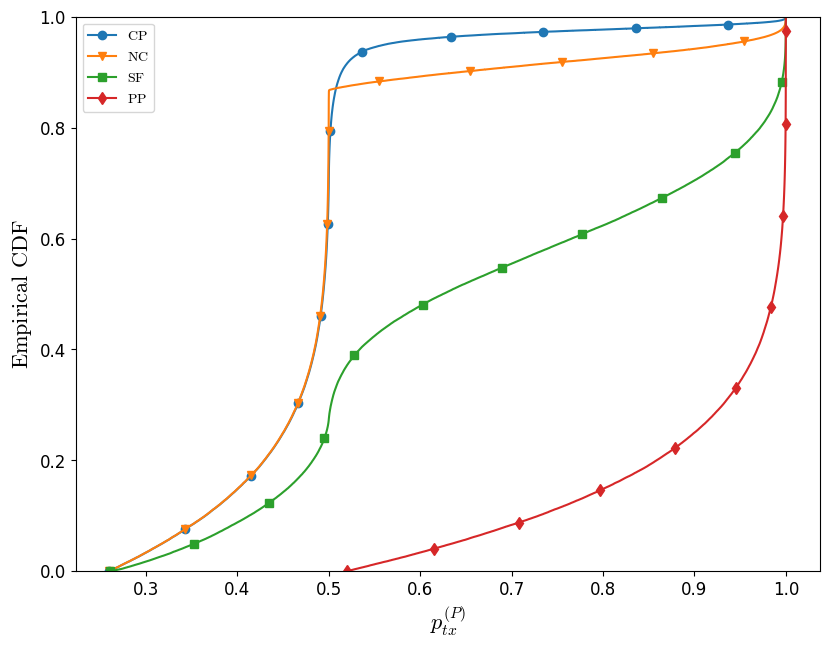
\includegraphics[width=0.8\linewidth]{compare-ptxp.png}
\caption{So sánh xác suất truyền tin tại PU giữa các chiến lược tối ưu khác nhau. $N=200000$}
\label{fig:Compare:ptxp}
\end{figure}

\subsection{Trong điều kiện xác suất truyền tin tương đồng}

Để đánh giá khách quan hiệu quả an toàn của PU giữa các chiến lược, phần tiếp theo sẽ trình bày kết quả so sánh giữa các chiến lược khi xác suất truyền tin tại PU sai khác nhau dưới $1\%$. Hình~\ref{fig:Compare:Sameptx:rlsf} phản ánh mức độ chênh lệch về $R_L^{(P)}$ đạt được tại hai chiến lược $SF$ và $NC$. Trong hình, phần giá trị dương theo trục hoành tương ứng với các trường hợp $R_L^{(P)}$ trong chiến lược $SF$ tốt hơn chiến lược $NC$. Có thể thấy trong hầu hết trường hợp, các giá trị chênh lệch đều rất gần $0$. Khi so sánh phần giá trị dương với phần giá trị âm, ta thấy có đa số các trường hợp mà chiến lược $SF$ (chiến lược hợp tác) giúp cải thiện hiệu năng an toàn so với $NC$ (chỉ có PU truyền tin). Như vậy, với cùng xác suất truyền tin, ngay cả khi SU chỉ ưu tiên tối ưu cho hiệu năng của mình thì việc hợp tác với SU cũng giúp PU cải thiện hiệu năng an toàn. Hình~\ref{fig:Compare:Sameptx:rlcp} cũng cho thấy kết quả tương tự khi so sánh giữa hai chiến lược $CP$ và $NC$. Song với trường hợp này, do chiến lược $CP$ ưu tiên tối ưu $R_L^{(P)}$ nên chênh lệch về hiệu quả an toàn so với chiến lược $NC$ là cao hơn rõ rệt.

\begin{figure}
\centering
\captionsetup{justification=centering}

\begin{subfigure}{0.8\textwidth}
\centering
\captionsetup{justification=centering}
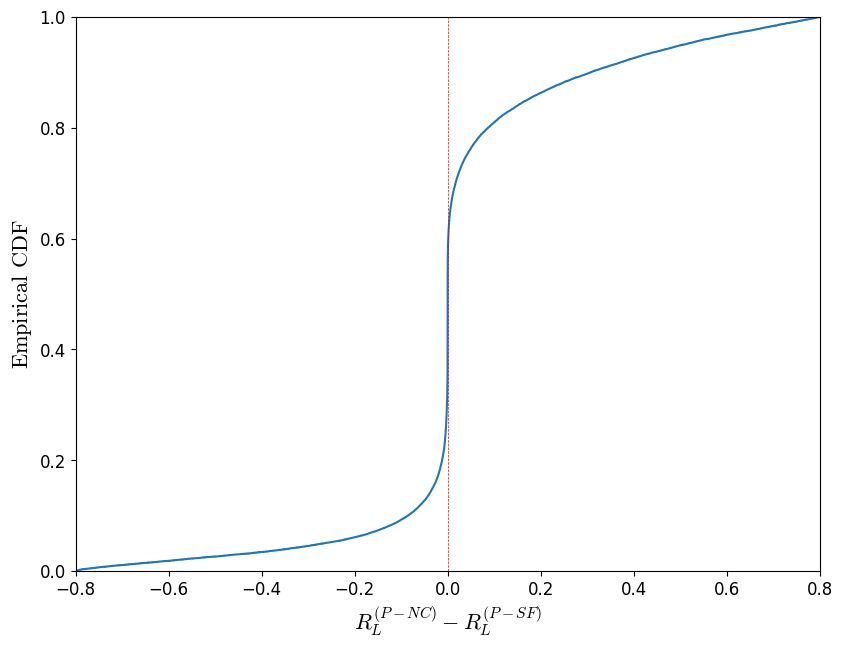
\includegraphics[width=1\linewidth]{Figures/compare-sameptx-sf.png}
    \caption{Giữa $SF$ và $NC$}
    \label{fig:Compare:Sameptx:rlsf}
\end{subfigure}

\begin{subfigure}{0.8\textwidth}
\centering
\captionsetup{justification=centering}
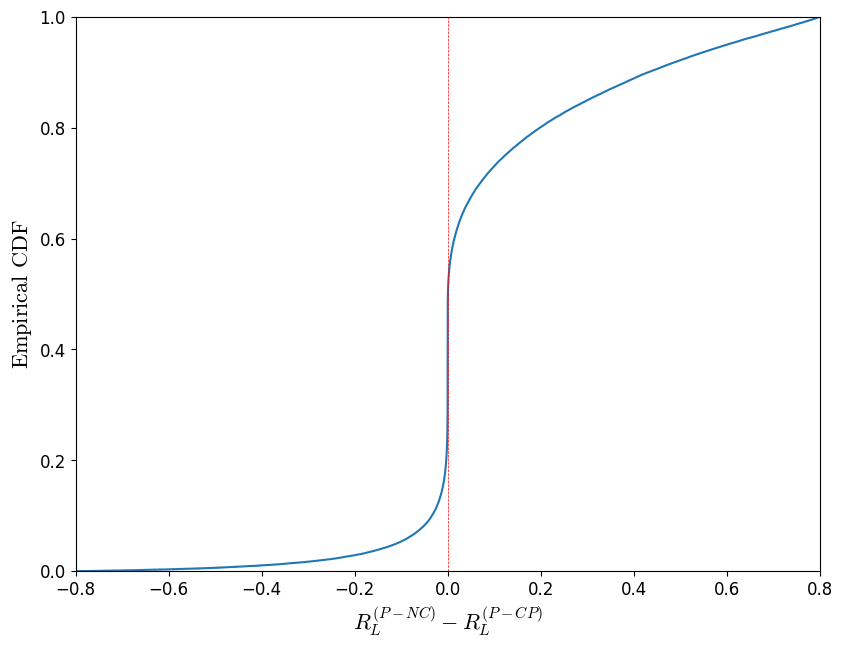
\includegraphics[width=1\linewidth]{Figures/compare-sameptx-cp.png}
\caption{Giữa $CP$ và $NC$}
\label{fig:Compare:Sameptx:rlcp}
\end{subfigure}
\caption{So sánh tốc độ lộ thông tin giữa các chiến lược trong các trường hợp xác suất truyền tin tại PU tương đồng nhau. $N=50000$}
\end{figure}

\subsection{Trong điều kiện kênh truyền nghe lén khác nhau}

Với mong muốn thấy rõ lợi ích của truyền tin hợp tác, phần này đánh giá các chiến lược trong trường hợp điều kiện kênh truyền nghe lén khác nhau. Cụ thể điều kiện này được đánh giá dựa trên so sánh khoảng cách từ $\text{PTx}$ và $\text{STx}$ tới kẻ nghe lén $\text{EAVP}$, tương ứng các đường truyền $h_{pe}$ và $h_{se}$. 

Hình~\ref{fig:Channel:Good} biểu diễn tốc độ lộ tin trung bình tại PU trong trường hợp bất lợi với kẻ nghe lén, vì lúc này can nhiễu từ $\text{STx}$ gây ra lớn hơn. Do đó, trong trường hợp này, giá trị $R_L^{(P)}$ trong các chiến lược đều tập trung vào dải giá trị nhỏ. Khi so sánh giữa hai chiến lược $SF$ và $NC$, ta thấy $NC$ thể hiện tốt hơn khi mật độ dải giá trị nhỏ của $R_L^{(P)}$ ($\left[0, 0.4\right]$) cao hơn. Mặt khác, mật độ dải giá trị lớn của $R_L^{(P)}$ ($\left[0.4, 0.8\right]$) trong chiến lược $NC$ lại cao hơn trong chiến lược $SF$. Điều này là do hiệu năng an toàn của $NC$ chỉ phụ thuộc vào $\Omega_{pe}$: dải giá trị nhỏ của $R_L^{(P)}$ tương ứng với $\Omega_{pe}$ nhỏ và dải giá trị lớn tương ứng với $\Omega_{pe}$ lớn. Trong khi đó, hiệu năng an toàn của $SF$ được tác động bởi cả $\Omega_{pe}$ và $\Omega_{se}$, nên kết quả ổn định hơn.

\begin{figure}
\centering
\captionsetup{justification=centering}

\begin{subfigure}{.8\textwidth}
\centering
\captionsetup{justification=centering}
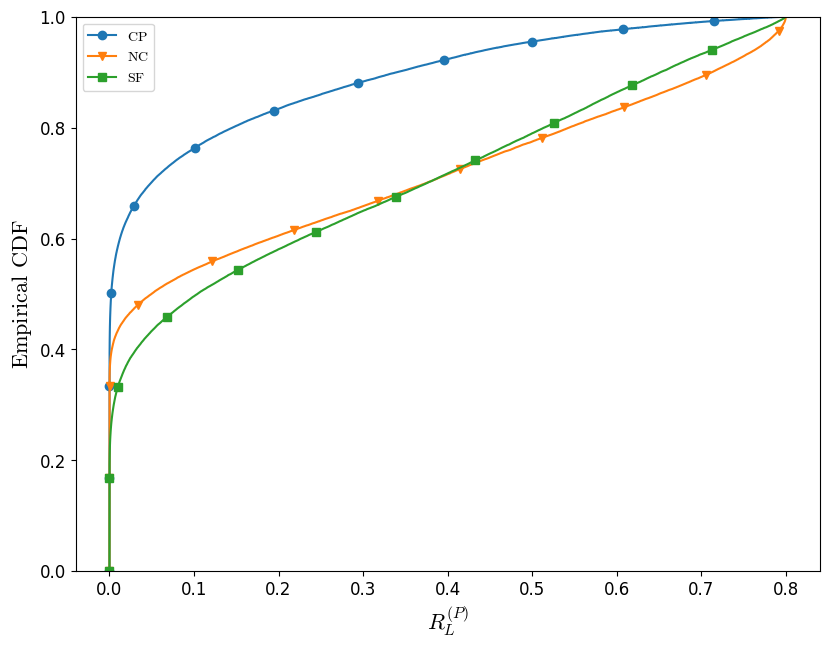
\includegraphics[width=1\linewidth]{Figures/compare-channel-good.png}
\caption{$\Omega_{pe} < \Omega_{se}$}
\label{fig:Channel:Good}
\end{subfigure}

\begin{subfigure}{.8\textwidth}
\centering
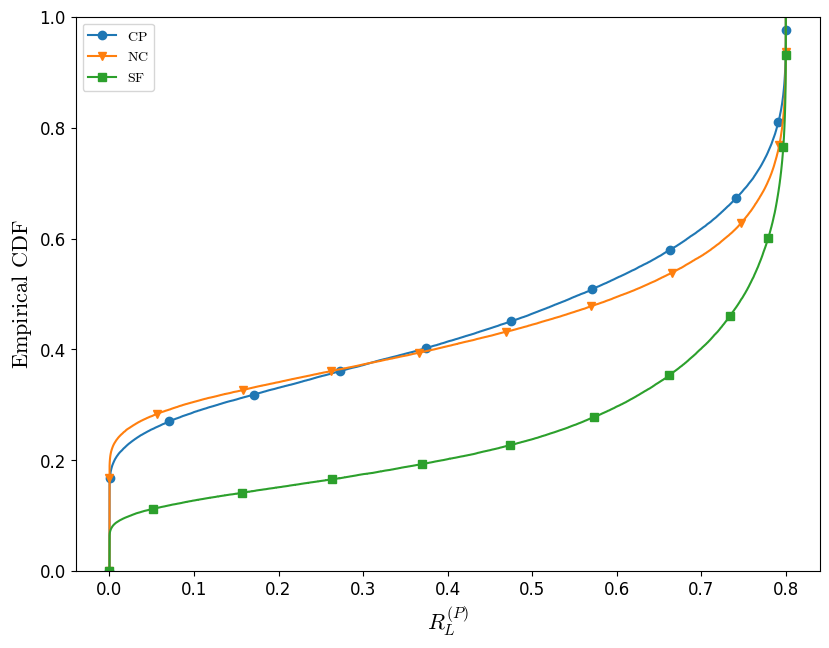
\includegraphics[width=1\linewidth]{Figures/compare-channel-bad.png}
\caption{$\Omega_{pe} > \Omega_{se}$}
\label{fig:Channel:Bad}
\end{subfigure}

\caption{So sánh tốc độ lộ thông tin giữa các chiến lược trong trường hợp điều kiện kênh truyền nghe lén khác nhau. $N=100000$}
\end{figure}

Khác với trường hợp trên, Hình~\ref{fig:Channel:Bad} biểu diễn tốc độ lộ tin trung bình tại PU trong trường hợp có lợi với kẻ nghe lén. Vì thế, giá trị $R_L^{(P)}$ lúc này tập trung vào dải giá trị lớn. Trong trường hợp này, $NC$ lại thể hiện là một chiến lược hiệu quả. Lý do là bởi hai chiến lược $CP$ và $SF$ không khai thác được nhiều lợi ích từ can nhiễu của SU. Tuy nhiên, tương tự như Hình~\ref{fig:Channel:Good}, khi so sánh giữa hai chiến lược $CP$ và $NC$, ta thấy việc hợp tác với SU giúp chất lượng truyền tin an toàn của PU ổn định hơn. Có thể thấy, trong điều kiện kênh truyền này, cơ hội mà SU được hợp tác truyền tin với PU là rất thấp, hoặc nếu được lựa chọn thì hiệu năng an toàn tại SU cũng không cao. 

\section{Hệ thống với nhiều người dùng thứ cấp}

Phần này trình bày kết quả liên quan đến mô hình mở rộng, trong đó hệ thống có nhiều SU cạnh tranh với nhau để được PU lựa chọn cùng truyền tin. Trước hết, phần này thực hiện đánh giá hiệu năng hệ thống theo tham số $\theta^{(S)}$ trong "bài toán cạnh tranh". Hình~\ref{fig:ThetaS:RLP} và Hình~\ref{fig:ThetaS:RLS} biểu diễn tốc độ lộ tin trung bình tại PU và SU ứng với các giá trị $\theta^{(S)}$ khác nhau. Kết quả cho thấy, khi $\theta^{(S)}$ càng tăng, tức yêu cầu về an toàn của SU càng thấp, thì hiệu quả an toàn tại PU càng cao. Tuy nhiên, ngay cả khi các ngưỡng $\theta^{(S)}$ có sự thay đổi lớn (chênh lệch $0.3$), giá trị $R_L^{(P)}$ không cho thấy sự thay đổi đáng kể. Điều đó cho thấy, điều kiện kênh truyền ảnh hưởng không nhỏ tới hiệu quả truyền tin của hệ thống. Ngay cả khi SU lựa chọn ưu tiên tối ưu cho hiệu năng an toàn của PU thì cũng không tăng đáng kể khả năng SU được PU lựa chọn hợp tác truyền tin.

\begin{figure}
\centering
\captionsetup{justification=centering}

\begin{subfigure}{.8\textwidth}
\centering
\captionsetup{justification=centering}
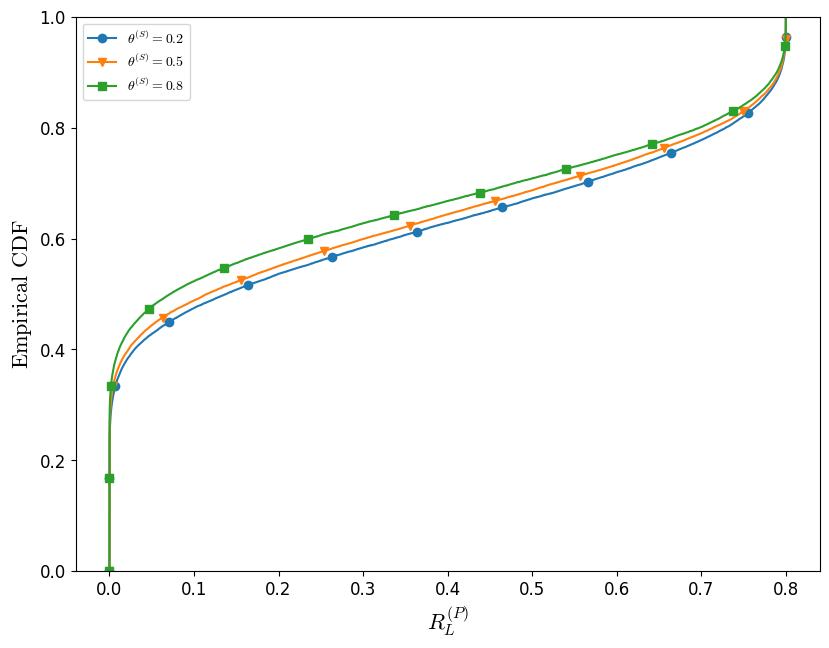
\includegraphics[width=1\linewidth]{Figures/thetas-rlp.png}
\caption{PU}
\label{fig:ThetaS:RLP}
\end{subfigure}

\begin{subfigure}{.8\textwidth}
\centering
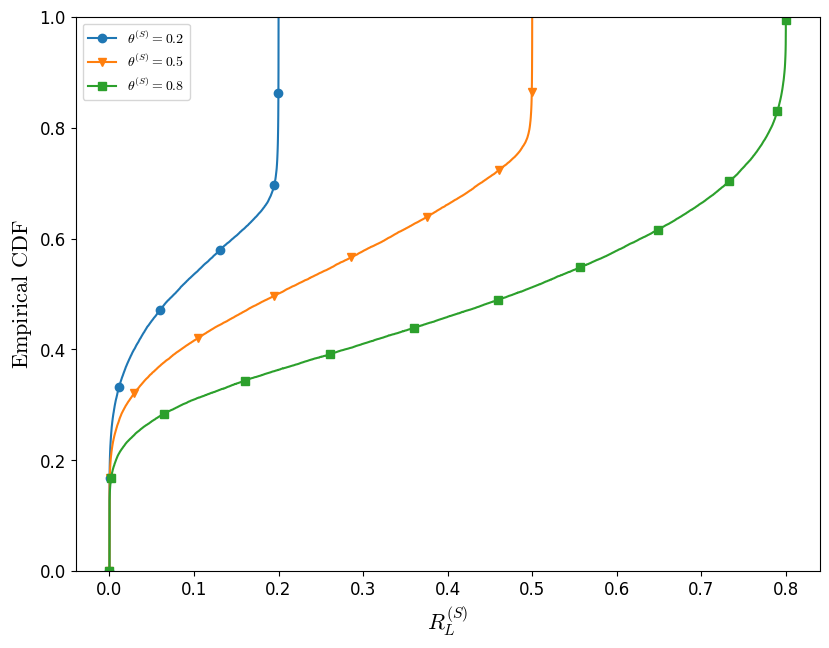
\includegraphics[width=1\linewidth]{Figures/thetas-rls.png}
\caption{SU}
\label{fig:ThetaS:RLS}
\end{subfigure}

\caption{So sánh tốc độ lộ tin trung bình của PU và SU trong bài toán cạnh tranh với các giá trị $\theta^{(S)}$ khác nhau. $N=50000$}
\end{figure}

Hình~\ref{fig:Multiuser:RLP} và Hình~\ref{fig:Multiuser:RLS} tương ứng biểu diễn tốc độ lộ tin trung bình tại PU và SU (SU được lựa chọn hợp tác) trong mô hình mở rộng với $M$ SU. Như đã đề cập, SU được lựa chọn là SU đề xuất chiến lược mang lại hiệu quả an toàn cao nhất cho PU. Trong thử nghiệm này, tất cả SU đều lựa chọn chiến lược ưu tiên tối ưu $R_L^{(P)}$, ứng với bài toán \eqref{competitive}, trong đó $\theta^{(S)} = 0.5$. Kết quả cho thấy, khi số lượng SU tăng lên thì hiệu quả an toàn tại PU được cải thiện rõ rệt. Đặc biệt, chỉ với hai SU, $M=2$, có đến khoảng $50\%$ cơ hội để tốc độ lộ tin trung bình của PU rất gần $0$ (với sai số $10^{-3}$), giá trị này lên tới $75\%$ khi $M=4$ và gần như chắc chắn khi $M=8$. Như vậy, mặc dù PU khó cải thiện hiệu năng an toàn với các chiến lược thiết kế của SU, nhưng khi số lượng SU lớn, PU có thể tăng đáng kể hiệu quả truyền tin an toàn. Mặt khác, hiệu quả an toàn của SU lại không suy giảm nhiều, thậm chí còn có phần cải thiện khi mật độ của dải giá trị lớn giảm đi.

\begin{figure}
\centering
\captionsetup{justification=centering}

\begin{subfigure}{.8\textwidth}
\centering
\captionsetup{justification=centering}
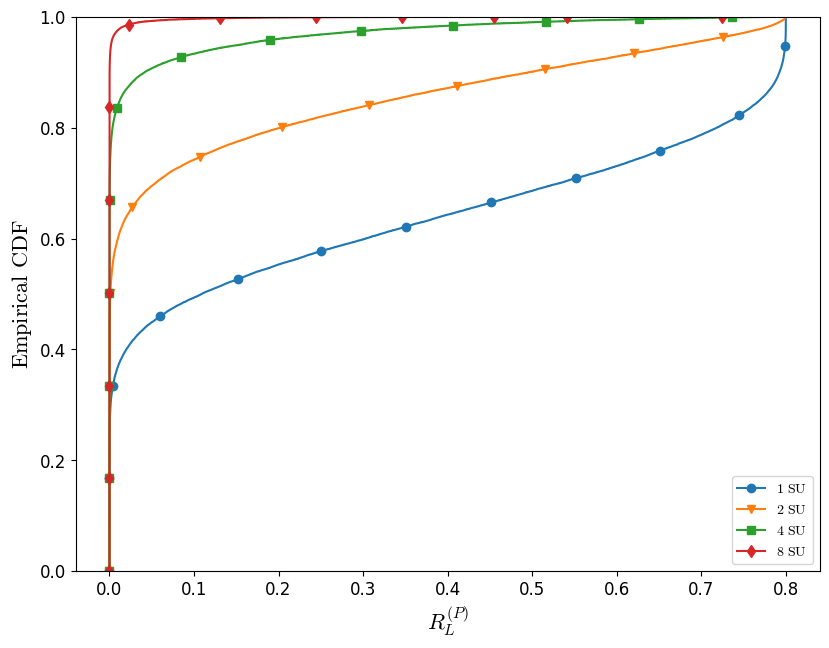
\includegraphics[width=1\linewidth]{Figures/multisus-rlp.png}
\caption{PU}
\label{fig:Multiuser:RLP}
\end{subfigure}

\begin{subfigure}{.8\textwidth}
\centering
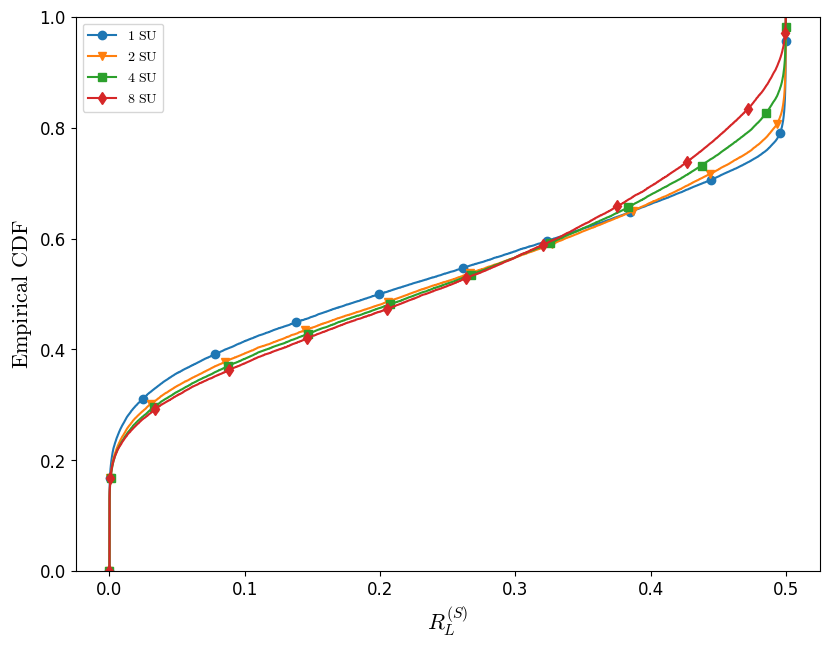
\includegraphics[width=1\linewidth]{Figures/multisus-rls.png}
\caption{SU được chọn}
\label{fig:Multiuser:RLS}
\end{subfigure}

\caption{Đánh giá tốc độ lộ tin trong mô hình nhiều SU cạnh tranh. $N=25000$}
\end{figure}

Với xác suất truyền tin của các bên trong mô hình mở rộng, kết quả thử nghiệm được thể hiện qua Hình~\ref{fig:Multiuser:PTXP} và Hình~\ref{fig:Multiuser:PTXS}. Kết quả cho thấy, khi số lượng SU tăng lên thì xác suất truyền tin tại PU cũng tăng lên đáng kể. Với $M=8$, có tới $75\%$ cơ hội để xác suất truyền tin của PU cao hơn $50\%$. Phía SU, xác suất truyền tin không cho thấy sự khác biệt rõ rệt. Như vậy, số lượng SU tăng lên không những giúp PU cải thiện hiệu quả truyền tin an toàn mà còn tăng xác suất truyền tin tại PU, trong khi đó, xác suất truyền tin tại SU không suy giảm. Từ các kết quả trên, có thể kết luận rằng, khi số lượng SU tăng lên, các hiệu năng an toàn của hệ thống ít chịu ảnh hưởng của điều kiện truyền tin.

\begin{figure}
\centering
\captionsetup{justification=centering}

\begin{subfigure}{.8\textwidth}
\centering
\captionsetup{justification=centering}
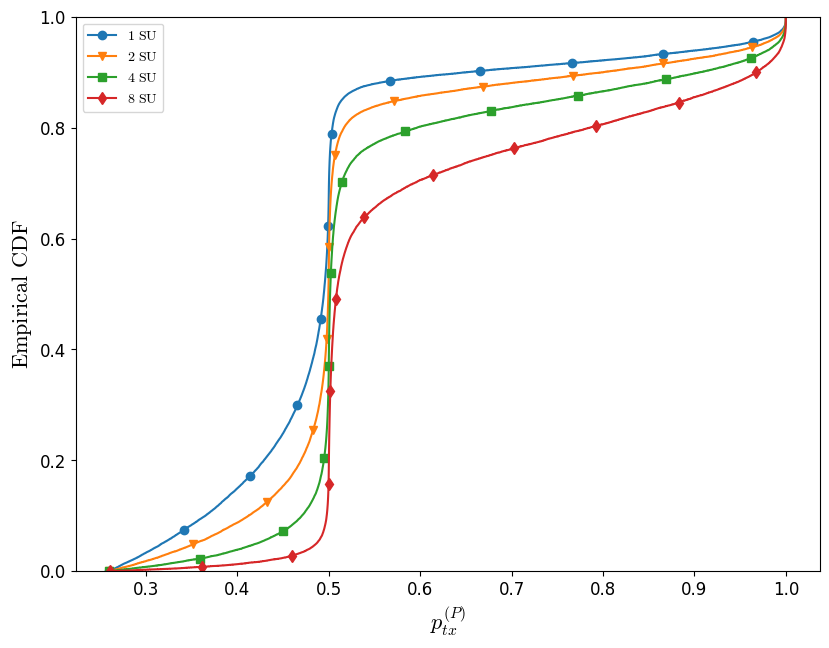
\includegraphics[width=1\linewidth]{Figures/multisus-ptxp.png}
\caption{PU}
\label{fig:Multiuser:PTXP}
\end{subfigure}

\begin{subfigure}{.8\textwidth}
\centering
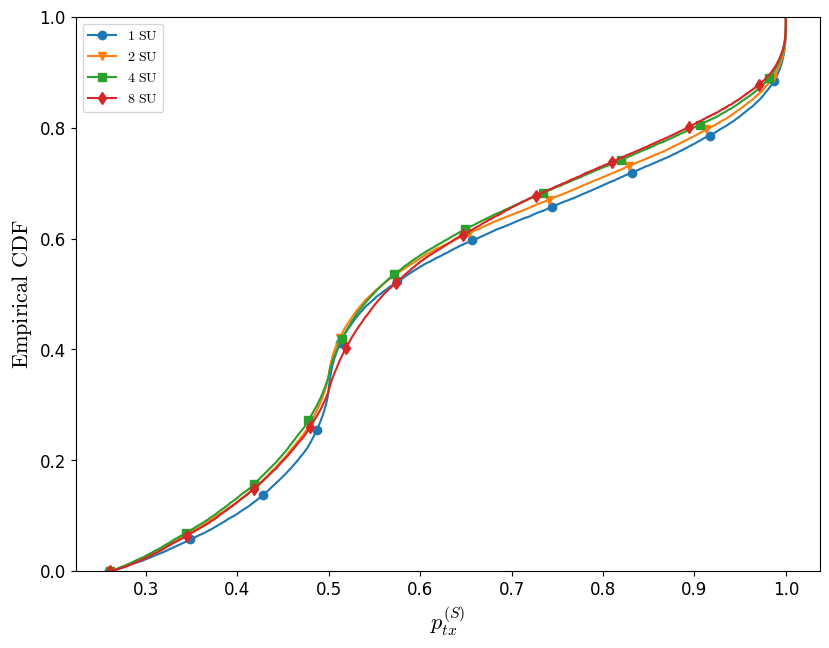
\includegraphics[width=1\linewidth]{Figures/multisus-ptxs.png}
\caption{SU được chọn}
\label{fig:Multiuser:PTXS}
\end{subfigure}

\caption{Đánh giá xác suất truyền tin trong mô hình nhiều SU cạnh tranh. $N=25000$}
\end{figure}

\section{Kết chương}

Chương này đã thực hiện đánh giá tính hiệu quả của các bài toán đề xuất thông qua các thử nghiệm với dữ liệu sinh ngẫu nhiên, phản ánh các điều kiện đường truyền khác nhau. Thông qua các kết quả, chương này cũng cho thấy ưu điểm và hạn chế của các chiến lược đề xuất. Đặc biệt, kết quả thử nghiệm với nhiều người dùng cho thấy tiềm năng của đề xuất mở rộng hệ thống khi giúp tăng hiệu quả an toàn và xác suất truyền tin cho các bên, đặc biệt là bên sơ cấp.

\end{document}